\section{Network Characteristics of Notification Services}
\label{sec:characterize-os}

Mobile operating systems provide OS level notification services to optimize network usage.
The Apple Push Notification service (APNs) and Google Cloud Messaging (GCM)~\cite{gcm} are used by iOS and Android applications respectively to receive notifications from the Internet.
In this section we show how \platname was used to compare the notification services of iOS and Android, and detailing it behavior in the wild. 

\subsection{Controlled Experiment on Factory Reset Devices}

We first detail the detail the behavior of notification services by performing a controlled experiment on \emph{factory-reset} devices. 
The objective of this experiment was to analyze notification services for devices that are used \emph{out of the box}, and detail the impact of device manufacturer, and pre-installed applications. 

For our experiment, we performed a \emph{factory reset} on an iPod Touch, an iPad, an iPhone, a Samsung Galaxy SIII, and a Google Nexus S Phone; the reset was performed after their batteries were fully charged. 
We then perform the initialization step and assigned a dummy email account as the primary account to each of these devices.
We then allowed these devices to connect to the Internet over \wifi through \platname and monitored the Internet traffic from these devices.
We then studied the impact of access technology by letting the iPhone and Samsung Galaxy SIII tunnel traffic through \platname using cellular networks. 

We observed that the traffic volume during the 24 hour periods varied from 19~KB to 97~KB depending on the devices. 
We classify APNS and GCM messages using the TCP port numbers mentioned in their specifications~\cite{gcm, apns}.
Because we did not run any applications in the foreground, notification messages were responsible for largest fraction of the traffic volume; the share was 35\% for Nexus S, 88\% for the Samsung SIII and around 50\% for each of the iOS devices. 
The share of DNS traffic varied from 10\% to 40\% for each of the devices while the other services contributed to less than 10\% of the traffic volume.
The only exception was the Samsumg Galaxy SIII which used location services that contributed to 26\% of 47~KB traffic volume generated by the device.

\begin{figure}
\centering
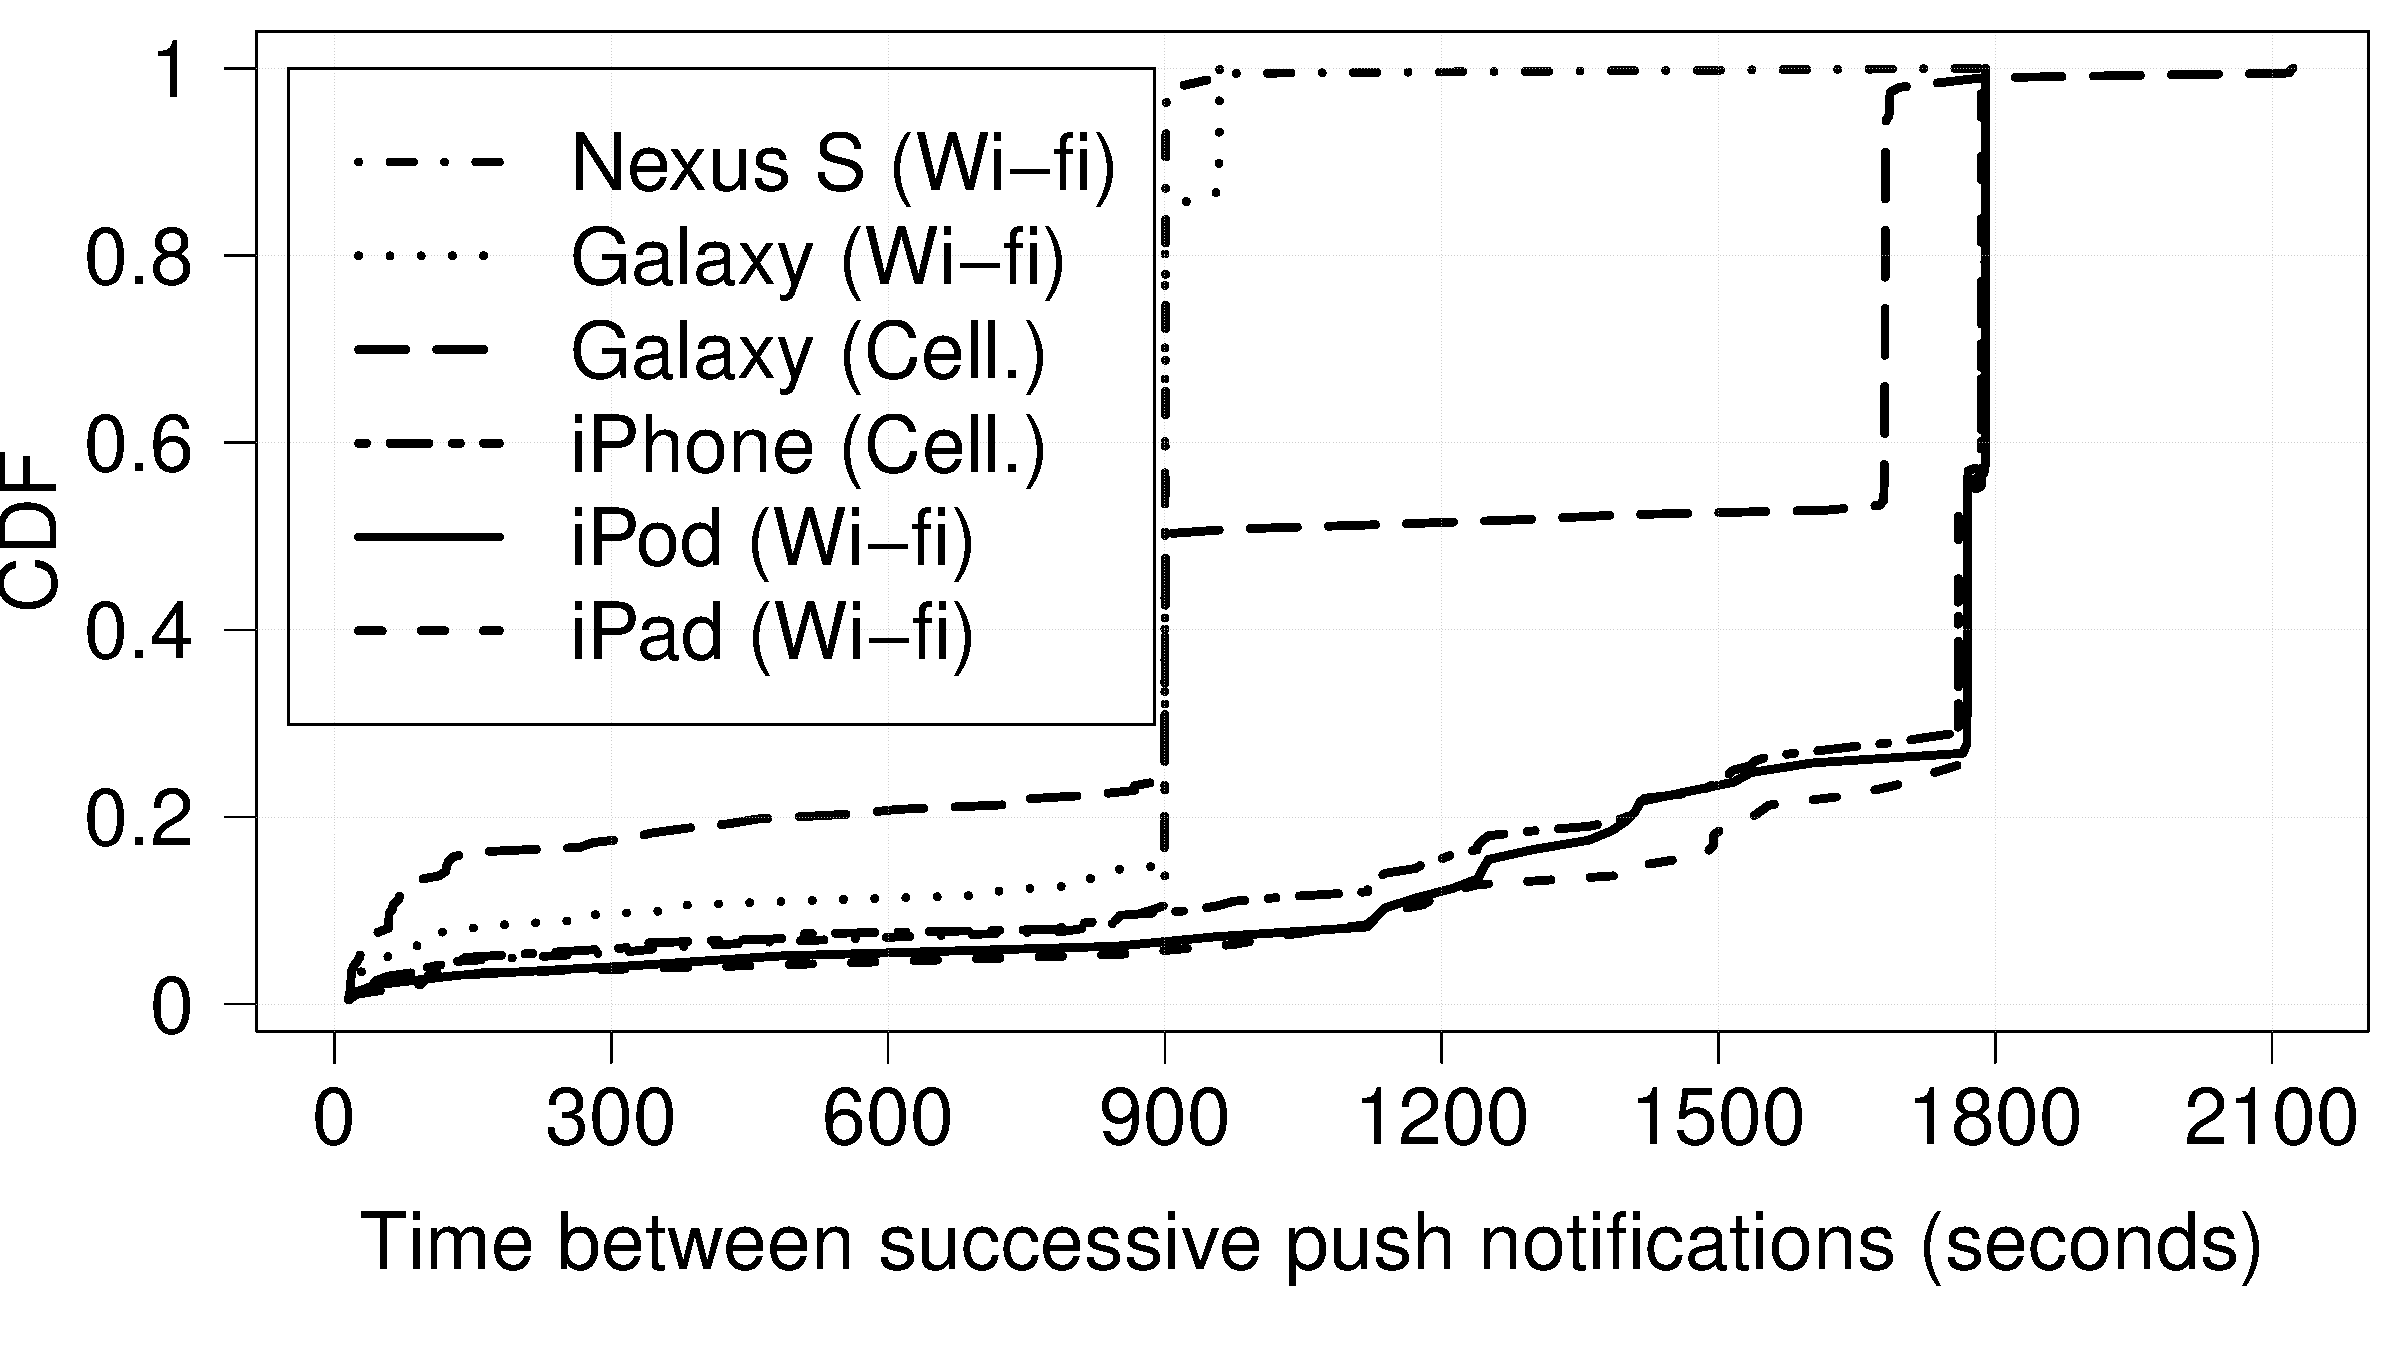
\includegraphics[width=\columnwidth]{plots/push_factoryreset_interarrival_distrib.pdf}
\caption{Inter-arrival time between notification messages after factory reset. \emph{The Android and iOS devices communicate with the notification server approximately once every 900~seconds and 1800 seconds respectively. The behavior of Android devices depends on the device, the pre-installed applications, and the access technology.}}
\label{fig:push-expt-interarrival}
\end{figure}

In \fref{fig:push-expt-interarrival} plot the time between successive messages sent by the notification servers on the ports assigned for notifications. 
We observe that the inter-arrival time between notifications for the Android devices is at least 900 seconds for more than 80\% of the notifications observed. 
The distribution of the inter-arrival time also depends on the access technology for the Samsung Galaxy SIII phone; we observe steps in the distribution for the SIII phone while we do not observe these steps when the same phone uses \wifi. 
We do not observe this difference when the Nexus S phone used the cellular data connection; we do not present the figure due to lack of space. 
\tbd{AR: Why these difference -- which applications stop coming up and so on}.
For the iOS devices, we observe an inter-arrival time at least 1700~seconds for that more than 75\% of the notifications in \fref{fig:push-expt-interarrival}. 
We do not observe a significant difference between the inter-arrival times for the iPhone over cell and \wifi and we do not present these results due to lack of space. 

On analyzing the packets exchanged, we observe that  all Android flows with an inter-arrival time larger than 800 seconds consisted of an empty TCP packet sent by the device followed by a 25 byte payload sent by the server.
Similarly, all iOS flows with an inter-arrival time larger than 1500 seconds began with an TCP packet with a payload of 85 bytes sent by the device followed by the server responding with of a TCP packet of 37 byte payload.

In summary, we observe notifications consume very little data, less than 50~KB in 24 hours, on Android and iOS devices in their default state.
The large time between successive notifications and the small amount of data exchanged implies they consume very little power.
We also observe that iOS devices have a larger time between successive notifications compared to Android devices in the default state. 
Furthermore, the inter-arrival time between notifications for Android devices differs based on the device manufacturer and the access technology. 

\subsection{Notifications In The Wild} 

We now characterize our observations on the notifications we observed in the \mobWild dataset. 
The objective of this analysis was to detail the frequency, traffic volume, and source of the notification services. 

\begin{figure}
\centering
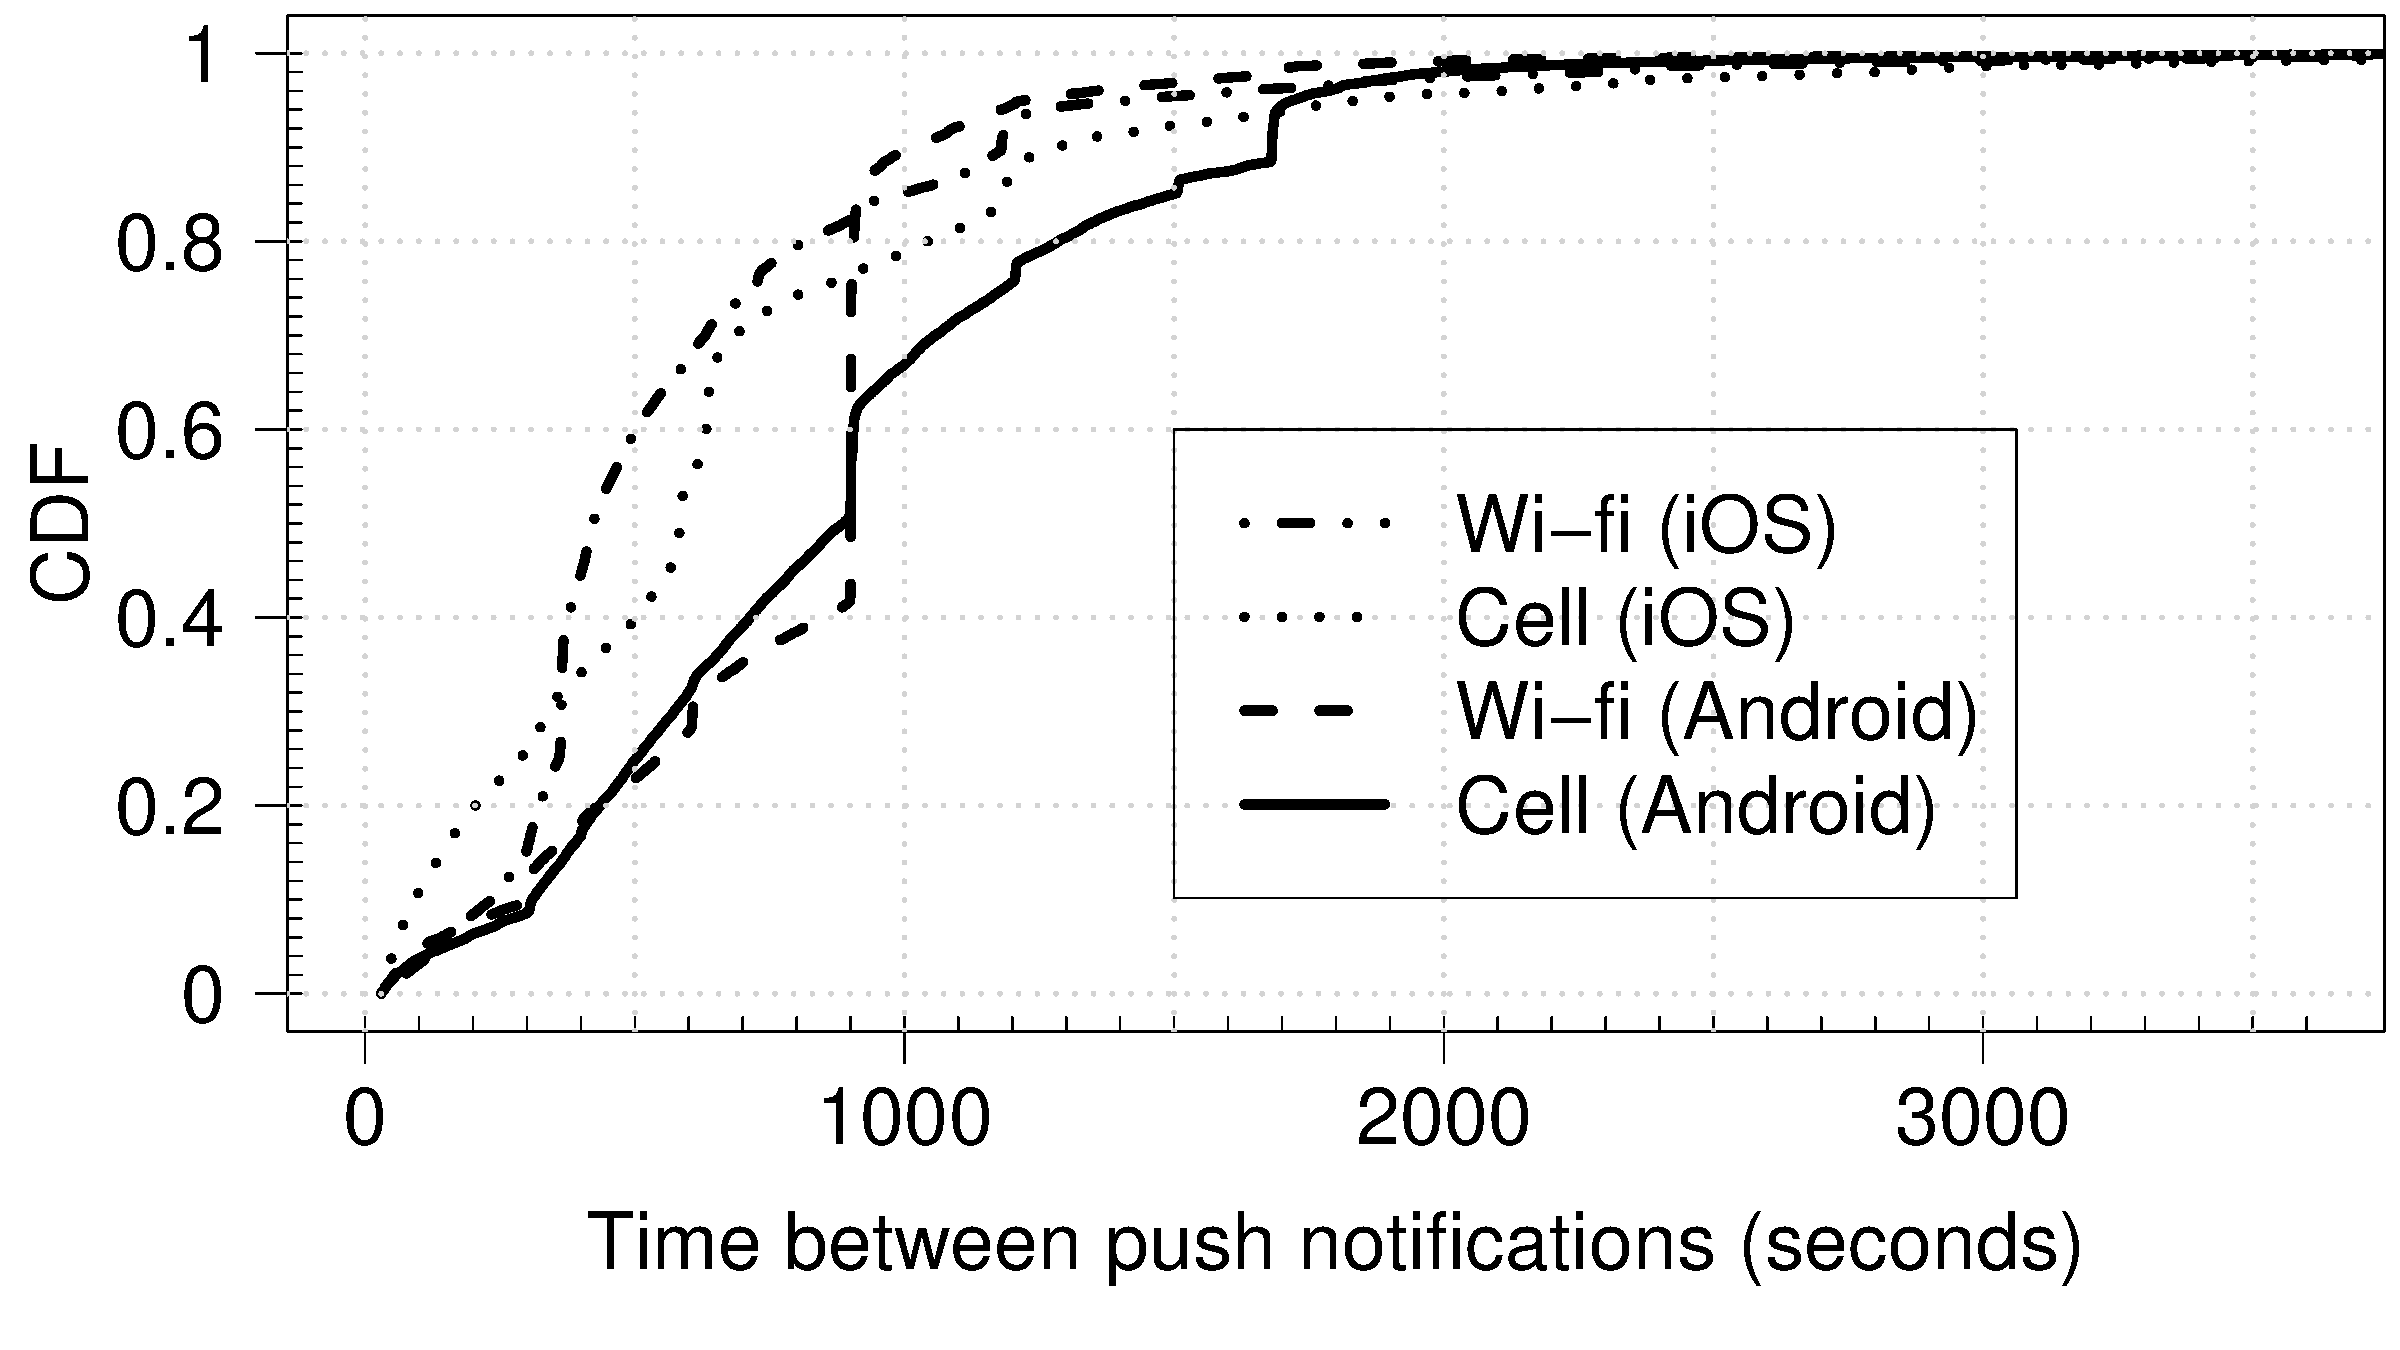
\includegraphics[width=\columnwidth]{plots/push_compare_os_tech_wild_distrib.pdf}
\caption{Distribution of the time between push notification messages in the wild. \emph{The frequency of push notification messages is higher for the iOS devices in our dataset compared to the Android devices. Notification messages are less frequent over cellular networks compared to Wi-Fi networks.}}
\label{fig:push-wild-compare-ostech}
\end{figure}

%The advantage of \platname is that it allows for direct comparison between devices across and their behavior across access technologies. 
To analyze the frequency of notification messages, we plot the distribution of the time between successive push notification messages for Android and iOS devices over cellular and \wifi networks in \fref{fig:push-wild-compare-ostech}.
In \fref{fig:push-wild-compare-ostech} we observe that a higher time between push notifications over cellular networks in comparison to \wifi networks for iOS and Android devices.  
We also observe the Android devices in our dataset receive notifications less frequently compared to the iOS devices in our dataset. 
We also observe a heavy tail for the time between notification messages which implies potentially long idle intervals.
\tbd{Correlation between time between notification messages and size of the next idle time observed?}


\begin{figure}
\centering
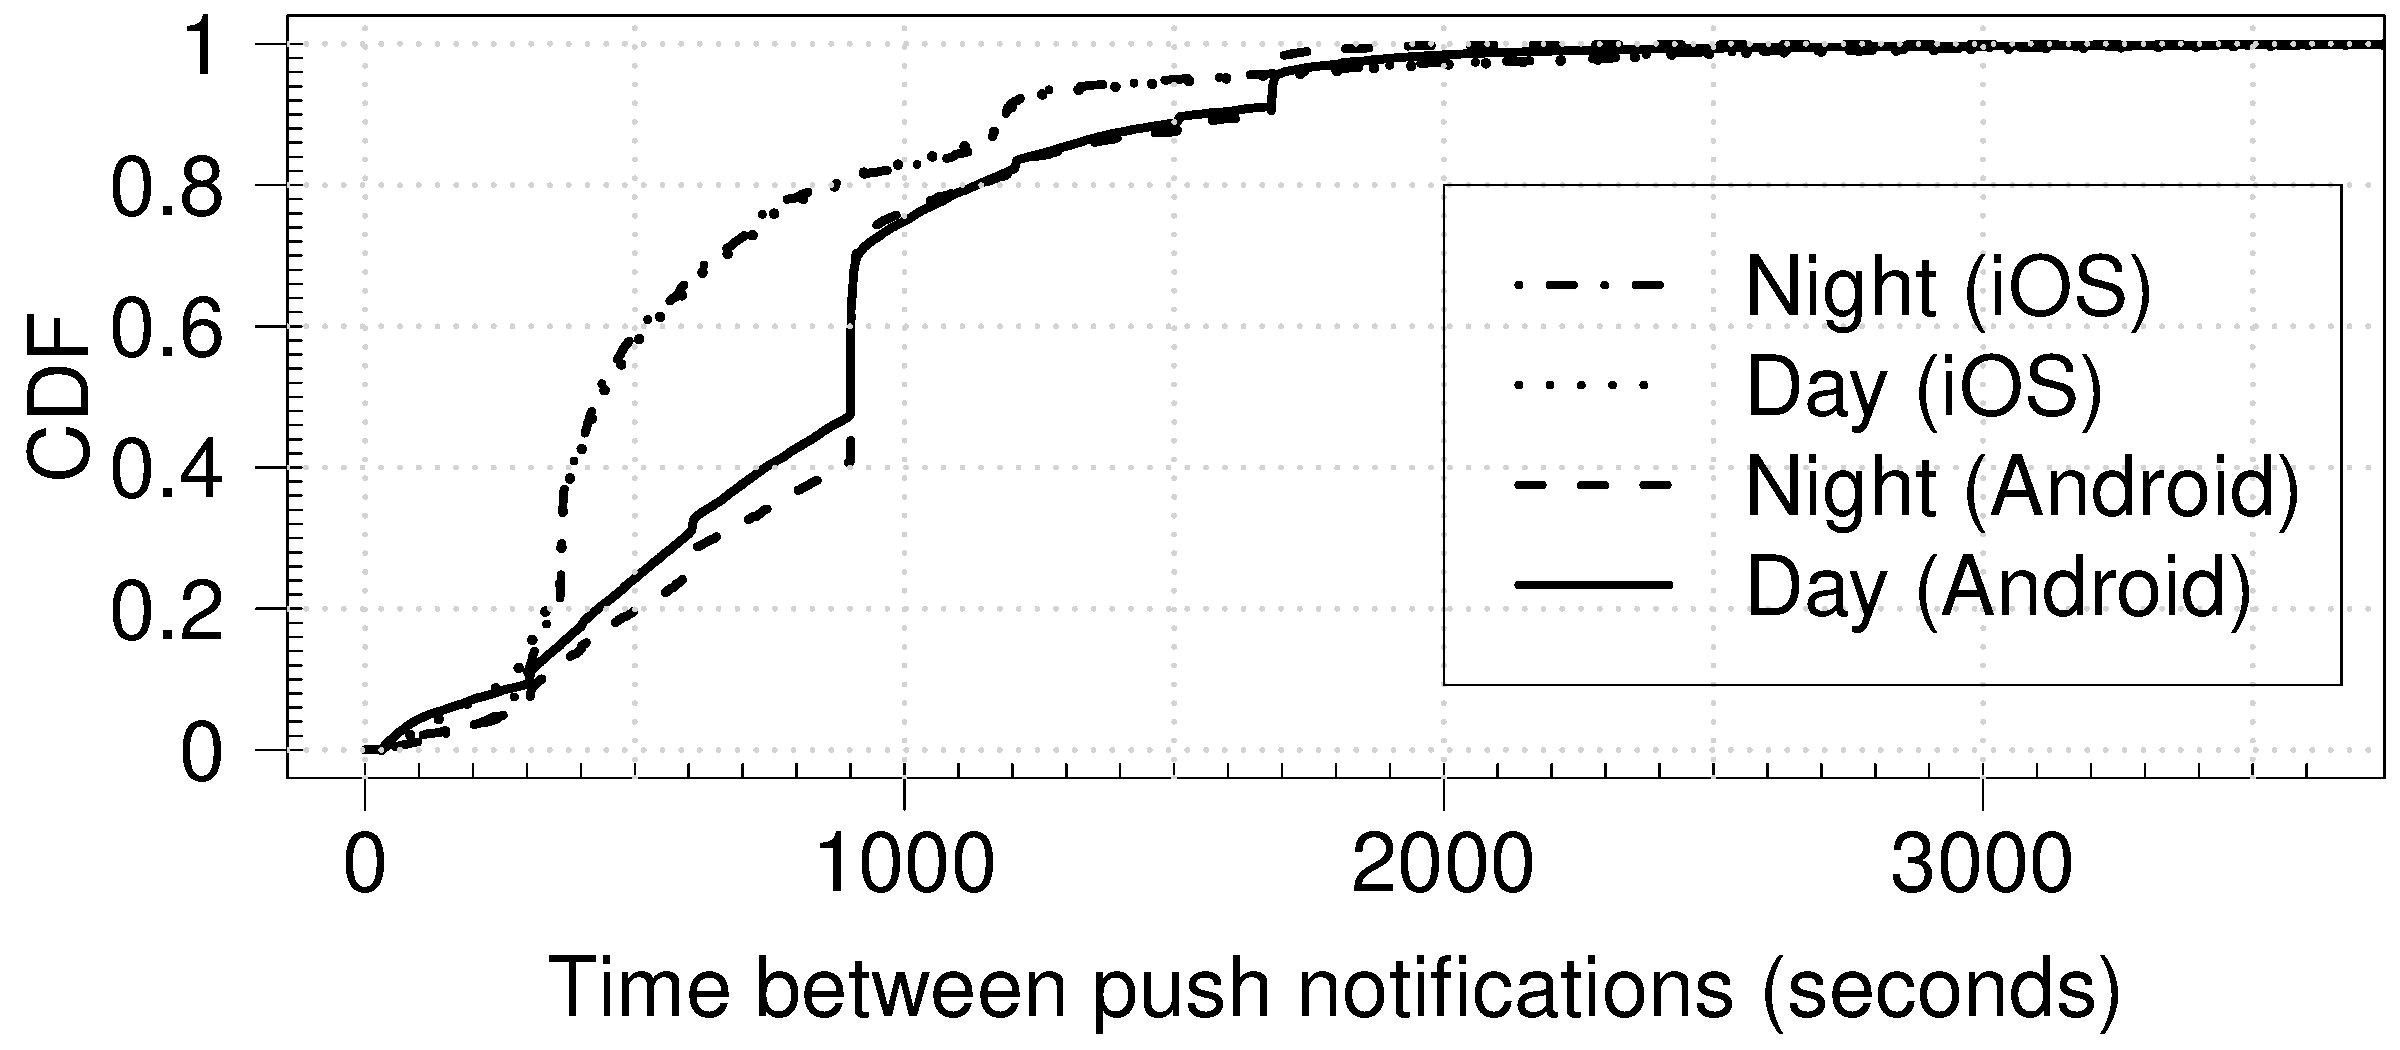
\includegraphics[width=\columnwidth]{plots/push_compare_diurnal_wild_distrib.pdf}
\caption{Impact of time-of-day on the push notifications. \emph{The rate of push notifications is agnostic of the time of the day for iOS devices.}}
\label{fig:push-wild-diurnal}
\end{figure}

The notification messages could be in response to user actions, for example, a mail server might receive a notification of a new message.
To analyze this impact, we notification messages received during two time intervals: from midnight to 6 am (night), and from 6 am to midnight (day). 
In \fref{fig:push-wild-diurnal}, we plot the distribution between successive notification messages for these two intervals. 
We observe that the Android and iOS devices appear to be agnostic of the time of the day. 
The iOS devices (from verion 6.0) come with a feature called \emph{Do Not Disturb (DND)} that does raise notification alarms on receiving notifications during specific time periods. 
We observe notification messages were received by the device that had enabled this feature during the intervals their users had configured as \emph{Do Not Disturb}.

\begin{figure}
\centering
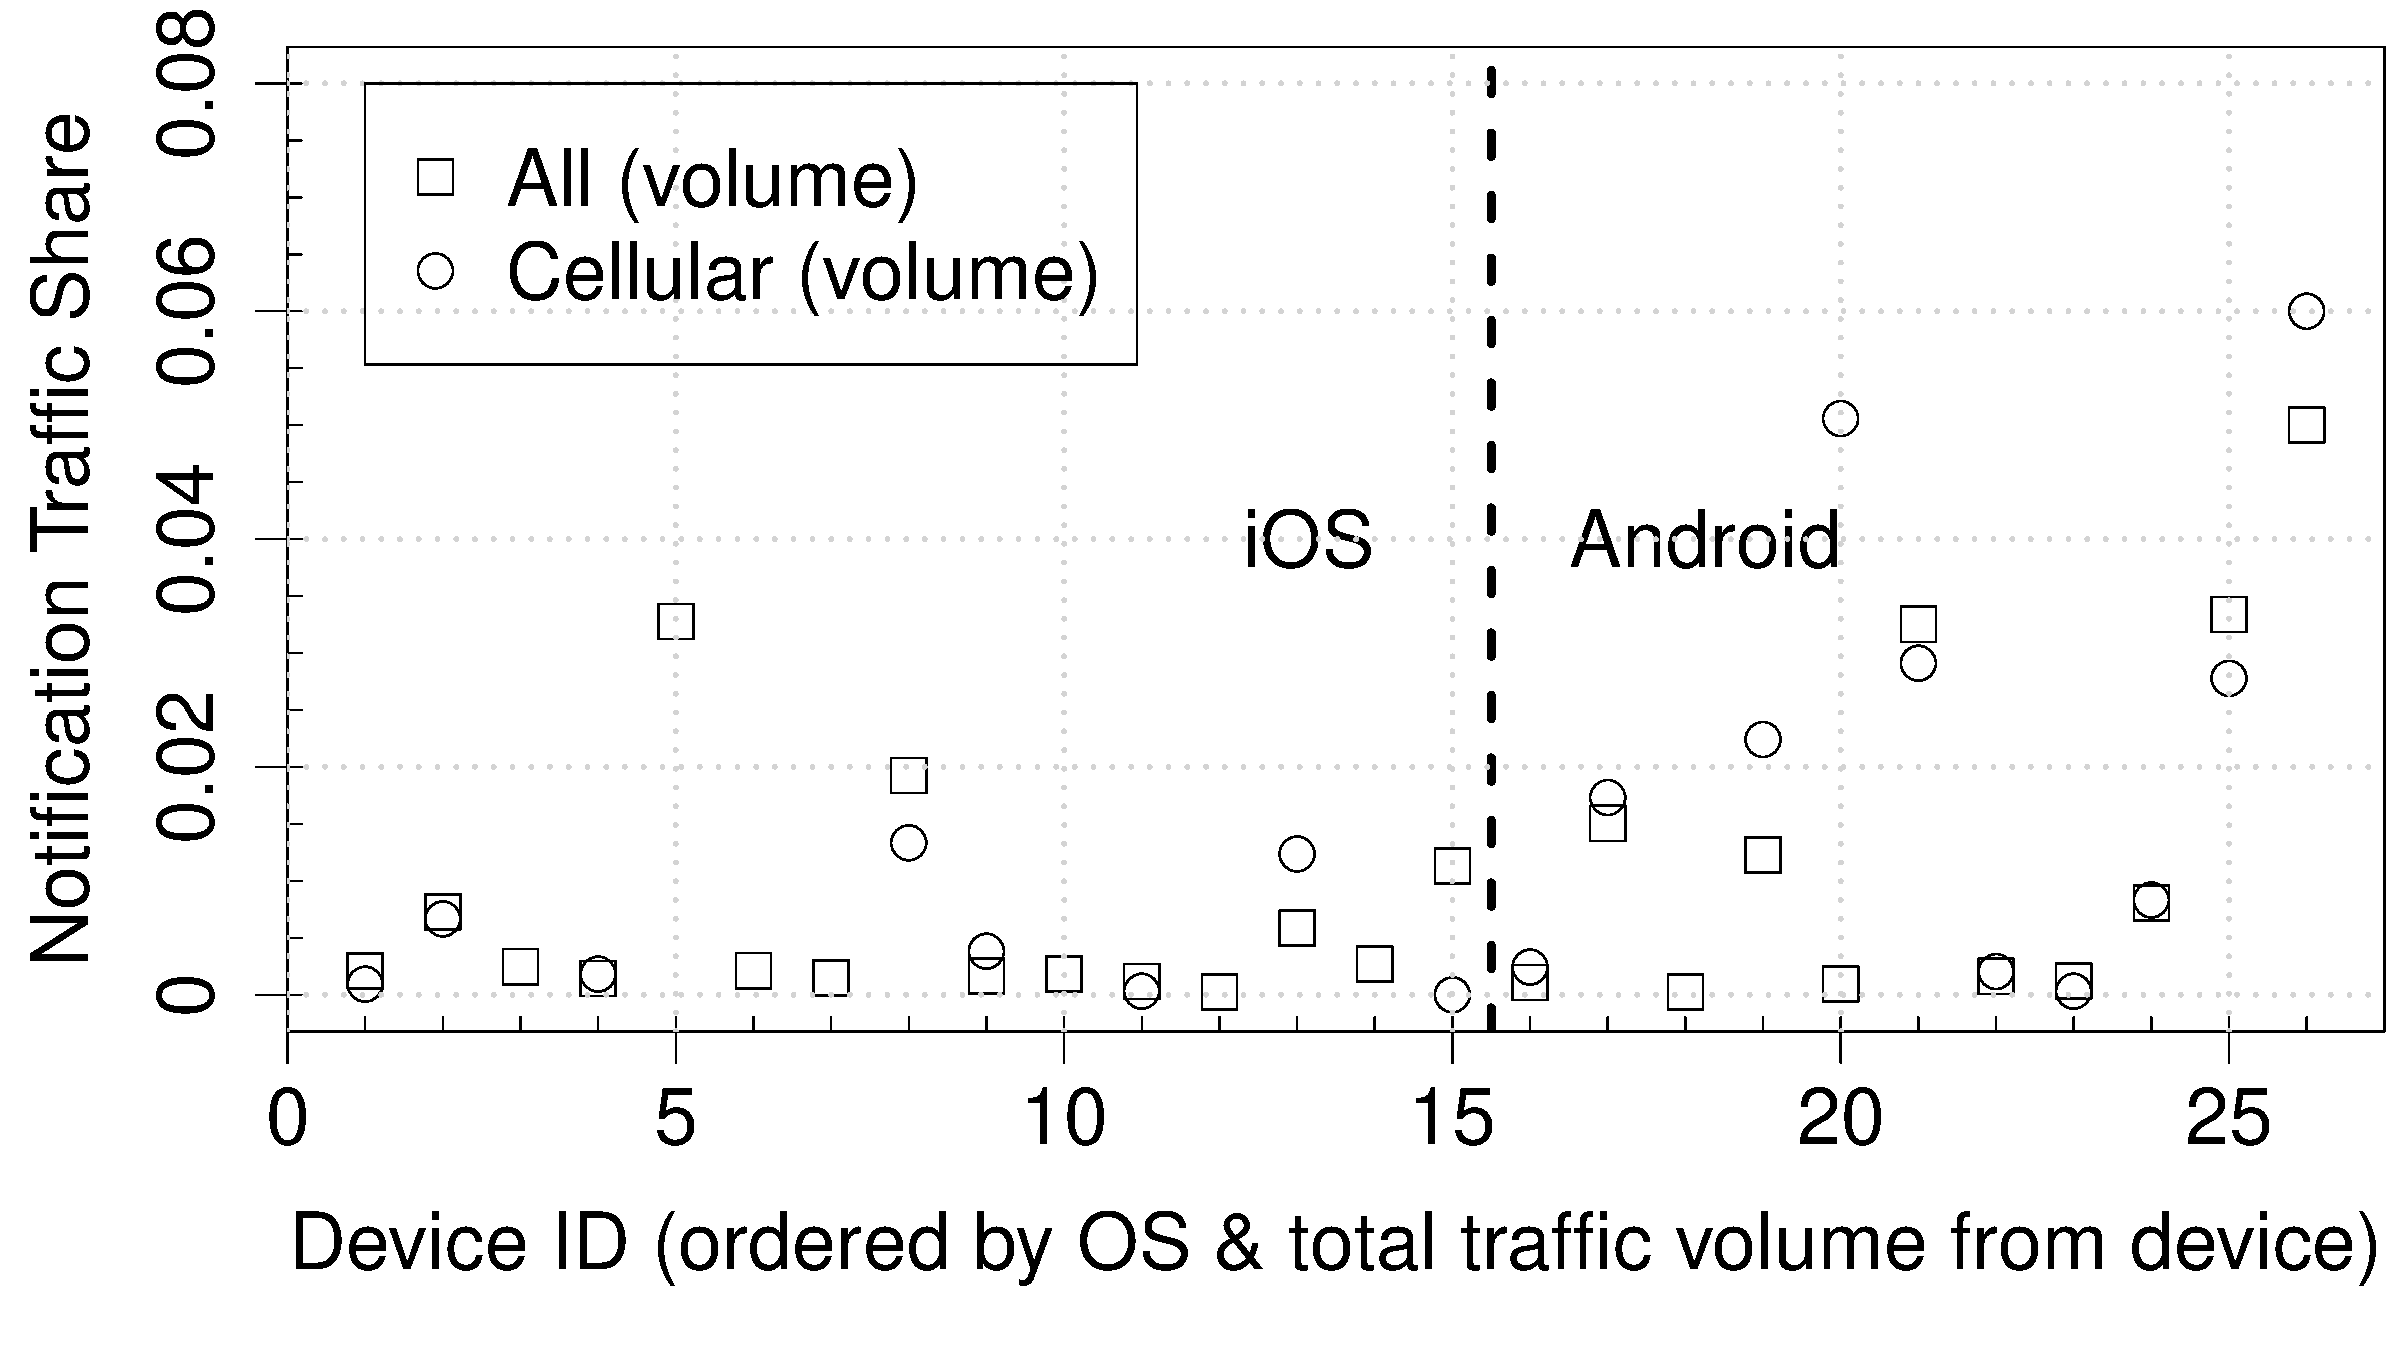
\includegraphics[width=\columnwidth]{plots/push_compare_trafficshare.pdf}
\caption{Traffic share of push notifications. \emph{Push notifications are responsible for less than 5\% of the traffic volume on most devices.}}
\label{fig:push-traffic-share}
\end{figure}

To analyze the volume of notification messages, we plot the share of notification messages as a fraction of total traffic from the device in \fref{fig:push-traffic-share}.
We observe that the notification messages are responsible for less than 4\% of the traffic volume on most Android and iOS devices. 
In \fref{fig:push-traffic-share}, we also plot the share of notification messages when the device exchanged data over cellular networks. 
We observe that there is no significant difference in the traffic share of notification messages when the device used cellular traffic. 
\tbd{Why do we care?}

To further analyze the source of the notification messages we analyzed the DNS lookups that were performed before the connections for receiving notification messages was established. 
We observed that the servers that pushed content to iOS devices correspond to the DNS requests that match the pattern \emph{*courier.push.apple.com} and \\ \emph{*courier-push-apple.com.akadns.net}.
For the android devices we observe that the DNS requests match the pattern\\ \emph{*talk.google.com}. 

In summary, we detail the behavior of the notification services using controlled experiments and the \mobWild dataset.  
We observe that push notifications consume a small fraction of the data and exhibit a heavy tail for the time between successive messages. 
We also observe that the frequency of notification messages was agnostic of the time of the day. 
Furthermore, notification messages were received by iOS devices even during the time interval the users had configured \emph{Do Not Disturb.}


% \begin{packedenumerate}
% \item How frequently do Push notifications take place in the wild?
% \item What is the impact of access technology on push notifications?
% \item What is the impact of the time of the day?
% \item What is the volume of push notification traffic?
% \item From which hosts are these notifications received?
% \end{packedenumerate}

%\subsection{Discussion}




% OLD TABLE WITHOUT IPHONE
% \begin{table}
% \begin{small}
% \begin{tabular}{|c|c|c|c|c|}
% \hline
% \multirow{2}{*}{\bf Application} & \multicolumn{4}{c|}{\bf Traffic Share in the first 24 hours}\tabularnewline
% \cline{2-5}
%      & iPad & iPod & Galaxy SIII & Nexus \tabularnewline
%      & (19 KB) & (21 KB) & (47 KB)& (97 KB)  \tabularnewline
% \hline
% Notifications & 0.54 & 0.53 & 0.35 & 0.88 \tabularnewline
% \hline
% Location & 0 & 0 & 0.26 & 0 \tabularnewline
% \hline
% SSL & 0 & 0 & 0.30 & 0.11 \tabularnewline
% \hline
% Mail & 0.05 & 0.07 & 0 & 0 \tabularnewline
% \hline
% HTTP & 0.13 & 0 & 0.09  & 0 \tabularnewline
% \hline
% UDP & 0.28 & 0.40 & 0.01 & 0.01 \tabularnewline
% \hline
% {\em total}& {\em 1.0} & {\em 1.0} & {\em 1.0} & {\em 1.0}\tabularnewline
% \hline
% \end{tabular}
% \end{small}
% \caption{Network usage in the first 24 hours after factory reset. \emph{Notifications contribute to the largest fraction of traffic volume across all devices.}}
% \label{tab:traffic-share-factory-reset}
% \end{table}

%While computing this distribution, we account the diversity in device usage in the following manner.
%For each device and each access technology we compute the 100 quantiles from 0.01 to 1.0 in steps of 0.01 of the time between successive push notifications. 
%We then use the median value of each quantile (from 0.01 to 1.0 in steps of 0.01) for a given access technology and operating system of the device.

% In \fref{fig:wild-inter-arrival-push} we present the time between successive push notifications for the 25 devices in our dataset. 
% As observed in \fref{fig:wild-cdf-push} we observe that the iOS devices receive push messages more frequently that the Android devices. 
% We also observe that the time between push notifications is higher for Android devices.
% The iOS devices prefer a cellular data connection for Push notification over \wifi \tbd{http://support.apple.com/kb/TS4264}. 
% However, in \fref{fig:wild-cdf-push} and \fref{fig:wild-cdf-push} despite this preference, we observe that the time between successive push notifications for iOS devices is higher over cellular networks in comparison to \wifi networks.  
% We observe that \tbd{SSL traffic} to mail servers was followed \tbd{x\%} after push notifications.
% This implies that higher usage of the device over \wifi may result in a higher number of notificatons received. 
% In \fref{fig:wild-inter-arrival-push}, device ID 
%Only if the cellular connection is not available or viable will the device switch to Wi-Fi for APNs connections.
